\chapter{提案手法}

\section{Web文書を用いたクエリゆう度モデルの拡張}
前章で述べたスムージングを用いながら,Web文書による情報量の拡張を図る.式(7.1)にWeb文書を併用したクエリゆう度モデルの式を示す.

\begin{flalign}
    & P(w_i|\theta_d; \alpha; \mu; \nu) = \nonumber \\ 
    & \frac{\alpha}{\alpha+\mu+\nu} P(w_i|\theta_d)
    &+ \frac{\mu}{\alpha+\mu+\nu} P(w_i|\theta_D)
    &+ \frac{\nu}{\alpha+\mu+\nu} P(w_i|\theta_W)  
    \label{eq_expanddirichlet}
\end{flalign}

ここで $P(w_i│θ_W)$はWeb文書集合 $W$ 内での語 $w_i$ の生起確率である.同様に $P(w_i│θ_D)$ は文書コレクション $D$ 内,$P(w_i│θ_d)$ は検索対象文書 $d$ 内の $w_i$ の生起確率である.また,$\alpha$, $\mu$, $\nu$はスムージングパラメータである.Web文書として,本研究では次節に倣い,各質問クエリから名詞情報を抽出して検索を行った結果を用いている. 

\subsection{Web 文書の取得}
Web文書の取得方法は,まず各クエリの単語に対してTF-IDF値を計算し,TF-IDF値のスコアの上位5単語を抽出する.そして,5単語から3単語を取り出す全て組み合わせおいて,Web検索を行い,各検索に対し10件のWeb文書を取得する.そのため,1クエリに対し,Web文書を100件取得した.最後に得られたWeb文書全てを,1つの巨大な文書とみなし,$P(w_i│θ_W)$ を計算し,式(7.1)で利用する.
ここでIDFの計算に文書コレクションを利用した.

\section{評価実験}
\subsection{実験条件}
提案手法の有用性を示すため,評価実験を行なった.Web文書をクエリ尤度モデルのスムージングに利用した式(8.1)を用いた場合(スムージングパラメータ: $\alpha$ = 0.5, $\mu$ = 0.3, $\nu$ = 0.2)とWeb文書を利用せず,スムージングに文書コレクションのみを利用した場合(スムージングパラメータ: $\alpha$ = 0.5, $\mu$ = 0.5, $\nu$ = 0.0)のMAP値を比較し,本手法の有用性を調べた.また,クエリの長さに応じたMAP値の変化も調査した.ここでクエリの長さは,クエリ内に存在する名詞の個数とする.クエリの長さに応じて4分割した際の各集合の条件を表7.1に纏める.

\begin{table}
    \centering
    \caption{クエリを分割したときに各集合}
    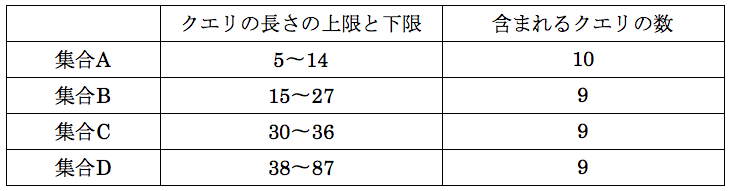
\includegraphics[width=7cm]{./image/query_set.png}
    \label{query_set}
\end{table}

\subsection{実験結果}
実験結果を図7.1に示す.

\begin{figure}
    \centering
    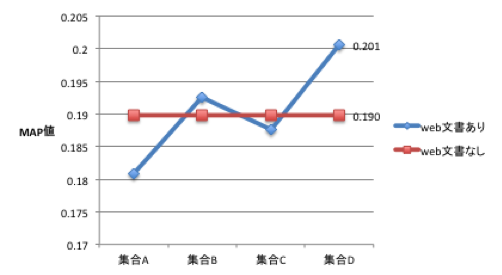
\includegraphics[width=7cm]{./image/web_result.png}
    \caption{Web文書を利用したときのMAP値}
    \label{web_result1}
\end{figure}

図7.1よりWeb文書を用いた本手法のMAP値の最大値は,Web文書を利用していない場合より高くなった.またクエリが長いほど本手法のMAP値は上昇した.これは,クエリが長いほど,文書コレクションだけではスムージングが対応できなくなり,Web文書によるスムージングが必要になるからだと考えられる.


\section{前後の部分文書の情報の加味}
NTCIR11のタスクでは,講演をより小さい単位で分割し,その一つを部分文書として,部分文書に対する検索精度を競う.部分文書に対して検索を行う場合,部分文書は文書長が短く,情報が少ないため,検索精度が低下すると考えられる.そのため本研究では,検索対象文書の周囲の文書も加味する事によって,文書検索精度の向上を図る.
まず,クエリと $i$ 番目の部分文書との類似スコアを $Score(i)$ とおく.この部分文書に対し,$i-N$ から $i+N$ 番目の部分文書を考慮する時,$ Score’(i)$ は式(9.1)で計算する.

\begin{equation}
    Score'(i) = \sum_{n=-N}^N w_n・Score(i + n) 
    \label{zengo1}
\end{equation}

ここで $w_n$は部分文書に付与する重みである.本研究では,適切な重みを調べるため,式(9.1)のnに応じた $w_n$ の変化が上に凸,比例,下に凸になるように,(i)ガウス重み,(ii)比例重み,(iii)反比例重みの3つを提案する.\\

\bf(i)ガウス重み \\

式(9.1)の $n$ に応じて,ガウス関数を利用した重みを付与する.ガウス重みは,分散パラメータ $\sigma$ を用いて式(9.2)で示す.

\begin{equation}
    w_n = \alpha⋅\exp⁡-(\frac{n}{2\sigma})^2
    \label{zengo2}
\end{equation}

ここで,$\alpha$ は $\sum_n w_n = 1$ となるように選ばれたスケールファクタである.また,分散パラメータ $\sigma$ は,部分文書の前後 $N$ 個を利用して式(9.3)のように定義した.

\begin{equation}
    \sigma = 0.3 * (\frac{2N+1}{2}) - 1 + 0.8
    \label{zengo3}
\end{equation}

\bf(ii)比例重み \\

式(9.1)の $n$ に応じて,比例的重みを付与する.比例重み $w_n$ を式(9.4)で定義した.

\begin{equation}
    w_n = N+1-|n|
    \label{zengo4}
\end{equation}

\bf(iii)反比例重み \\

式(9.1)の $n$ に応じて,反比例的重みを付与する.反比例重み $w_n$ を式(9.5)で定義した.

\begin{equation}
    w_n = 
    \begin{cases} 
        1 & (i = 0)\\ 
        \frac{1}{|i|+1} & (|i| > 0)
    \end{cases} 
    \label{zengo5}
\end{equation}

\section{評価実験}
\subsection{実験条件}
前後の部分文書にガウス重み・比例重み・反比例重みを用い,スコアを統合したときのMAP値の変化と前後の部分文書の数を変えたときのMAP値の変化を示す.スムージングパラメータは,$\alpha= 0.5, \mu= 0.5, \nu= 0.0$ である.

\subsection{実験結果}
実験結果を図9.1に示す.

\begin{figure}
    \centering
    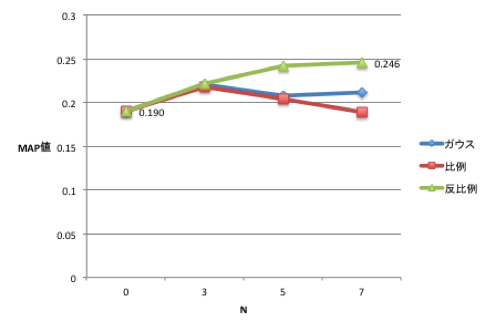
\includegraphics[width=7cm]{./image/zengo.png}
    \caption{前後の部分文書の加味したときのMAP値}
    \label{web_result1}
\end{figure}

実験結果として,図9.1から前後の部分文書を考慮するだけでもMAP値が上昇した.また,反比例重みを付与する事により,MAP値は最大0.246となり,前後の部分文書を考慮しないときよりもMAP値は0.056上昇した.この結果から,検索対象文書に対するスコアが重要であり,周囲の部分文書のスコアも少ない重みを付与して統合すると,検索精度が向上すると言える.